% !TeX spellcheck = fr_FR
\chapter{Chapitre 3 : Apprentissage machine}
\label{chap:3}

\section{Perceptron}
\label{sec:3.1}

Le perceptron est un algorithme d'apprentissage supervisé pour des problèmes de classification linéairement séparable (classifieur binaire). Le perceptron est la forme la plus simple de réseau de neurones possible. C'est un réseau qui a des entrées, un neurone comme couche intermédiaire et une sortie. On peut facilement le représenter sous forme de fonction qui mappe une entrée $\overrightarrow{X}$ (un vecteur de valeurs réelles) à une valeur de sortie $a$ (une valeur binaire) par un produit scalaire entre les poids $\overrightarrow{W}$ et les entrées $\overrightarrow{X}$ suivi d'une fonction d'activation.

{\Large
	\setlength{\abovedisplayskip}{-0.5cm}
	\begin{gather*}
		z = \sum_{i=0}^{N-1}{W_{i}X_{i}}
	\end{gather*}
}

\begin{figure}[H]
	\centering
	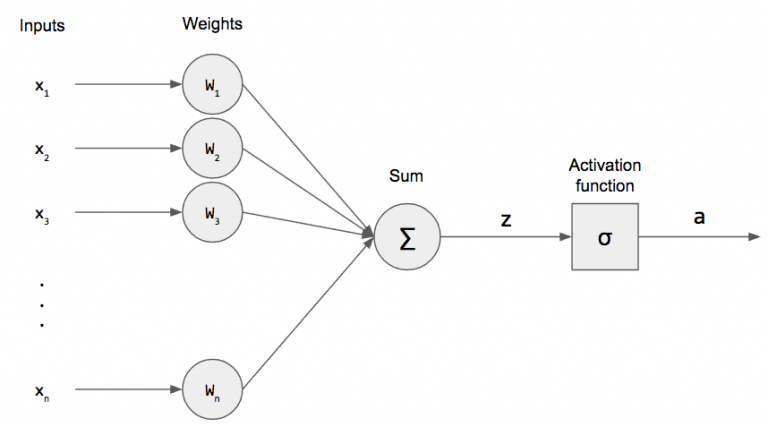
\includegraphics[width=0.7\linewidth]{perceptron}
	\caption[Perceptron]{Perceptron. Source : tiré de \textit{pythonmachinelearning.pro}, ref. URL02 / réalisé par \textsc{Deshpande} Mohit}
	\label{fig:perceptron}
\end{figure}

Les poids sont des valeurs réelles qui vont changer lorsque l’on va entrainer le perceptron. C’est-à-dire qu’on va lui faire classer une donnée dont on connait déjà la classe correcte puis une fois le classement effectué, on utilise une fonction de coût pour savoir de combien le perceptron s’est trompé. 

Par exemple l’erreur quadratique moyenne, où $Y_{i}$ représente la sortie actuelle, $\hat{Y}_{i}$ la sortie attendue et $N$ la taille.

{\Large
	\setlength{\abovedisplayskip}{-0.5cm}
	\begin{gather*}
		E[\overrightarrow{W}] = \frac{1}{N}\sum_{i=0}^{N-1}{(Y_{i} - \hat{Y}_{i})^2}
	\end{gather*}
}

Ensuite, grâce à la descente de gradient, nous pouvons trouver la valeur des poids qui minimisent la fonction de coût (l’erreur). Avec $\overrightarrow{W}$ le vecteur de poids, la mise à jour des poids $\overrightarrow{W}_t$ vers $\overrightarrow{W}_{t+1}$ peut être définie comme :

{\Large
	\setlength{\abovedisplayskip}{-0.5cm}
	\begin{gather*}
		\nabla E[\overrightarrow{W}] = [\frac{\partial E}{\partial W_{i}}] \\
		\Delta\overrightarrow{W} = -\eta\nabla E[\overrightarrow{W}] \\
		\overrightarrow{W}_{t+1} = \overrightarrow{W}_{t} + \Delta\overrightarrow{W}_{t}
	\end{gather*}
}

$\eta$ est le taux d’apprentissage, c’est un paramètre qui représente le pas que l’on va effectuer vers le minimum de la fonction de coût à chaque itération. C’est généralement un nombre assez petit, de sorte à ne pas sauter par-dessus le minimum de la fonction. Un taux d’apprentissage petit demande donc plus d’itérations pour converger et peut facilement se retrouver bloqué dans un minimum local.

Il est possible de rajouter une inertie (momentum) à la descente de gradient pour ne pas rester coincé dans un minimum local et de poursuivre la descente de gradient vers le minimum global de la fonction. Ce paramètre s'appelle généralement $\alpha$ (alpha) et il se situe entre zéro et un. Avec $\overrightarrow{W}$ le vecteur de poids et $\alpha$ l'inertie, la mise à jour des poids $\overrightarrow{W}_t$ vers $\overrightarrow{W}_{t+1}$ peut être définie comme :

{\Large
	\setlength{\abovedisplayskip}{-0.5cm}
	\begin{gather*}
		\nabla E[\overrightarrow{W}] = [\frac{\partial E}{\partial W_{i}}] \\
		\Delta\overrightarrow{W} = -\eta\nabla E[\overrightarrow{W}] \\
		\overrightarrow{W}_{t+1} = \overrightarrow{W}_{t} + \alpha\Delta\overrightarrow{W}_{t} + (1 - \alpha)\Delta\overrightarrow{W}_{t-1}
	\end{gather*}
}

\section{Fonction d'activation}
\label{sec:3.2}

Une fonction d'activation sert à définir la sortie d'un neurone par rapport à ses entrées, et donc de définir si ce neurone est activé ou non. Les fonctions d'activation sont généralement non linéaires mais il en existe plusieurs types.

{\Large
	\setlength{\abovedisplayskip}{-0.2cm}
	\begin{gather*}
		f(x) =
		\begin{cases}
			x & \: \text{si } x > 0 \\
			0 & \: \text{sinon}
		\end{cases}
	\end{gather*}
}

\begin{figure}[H]
	\centering
	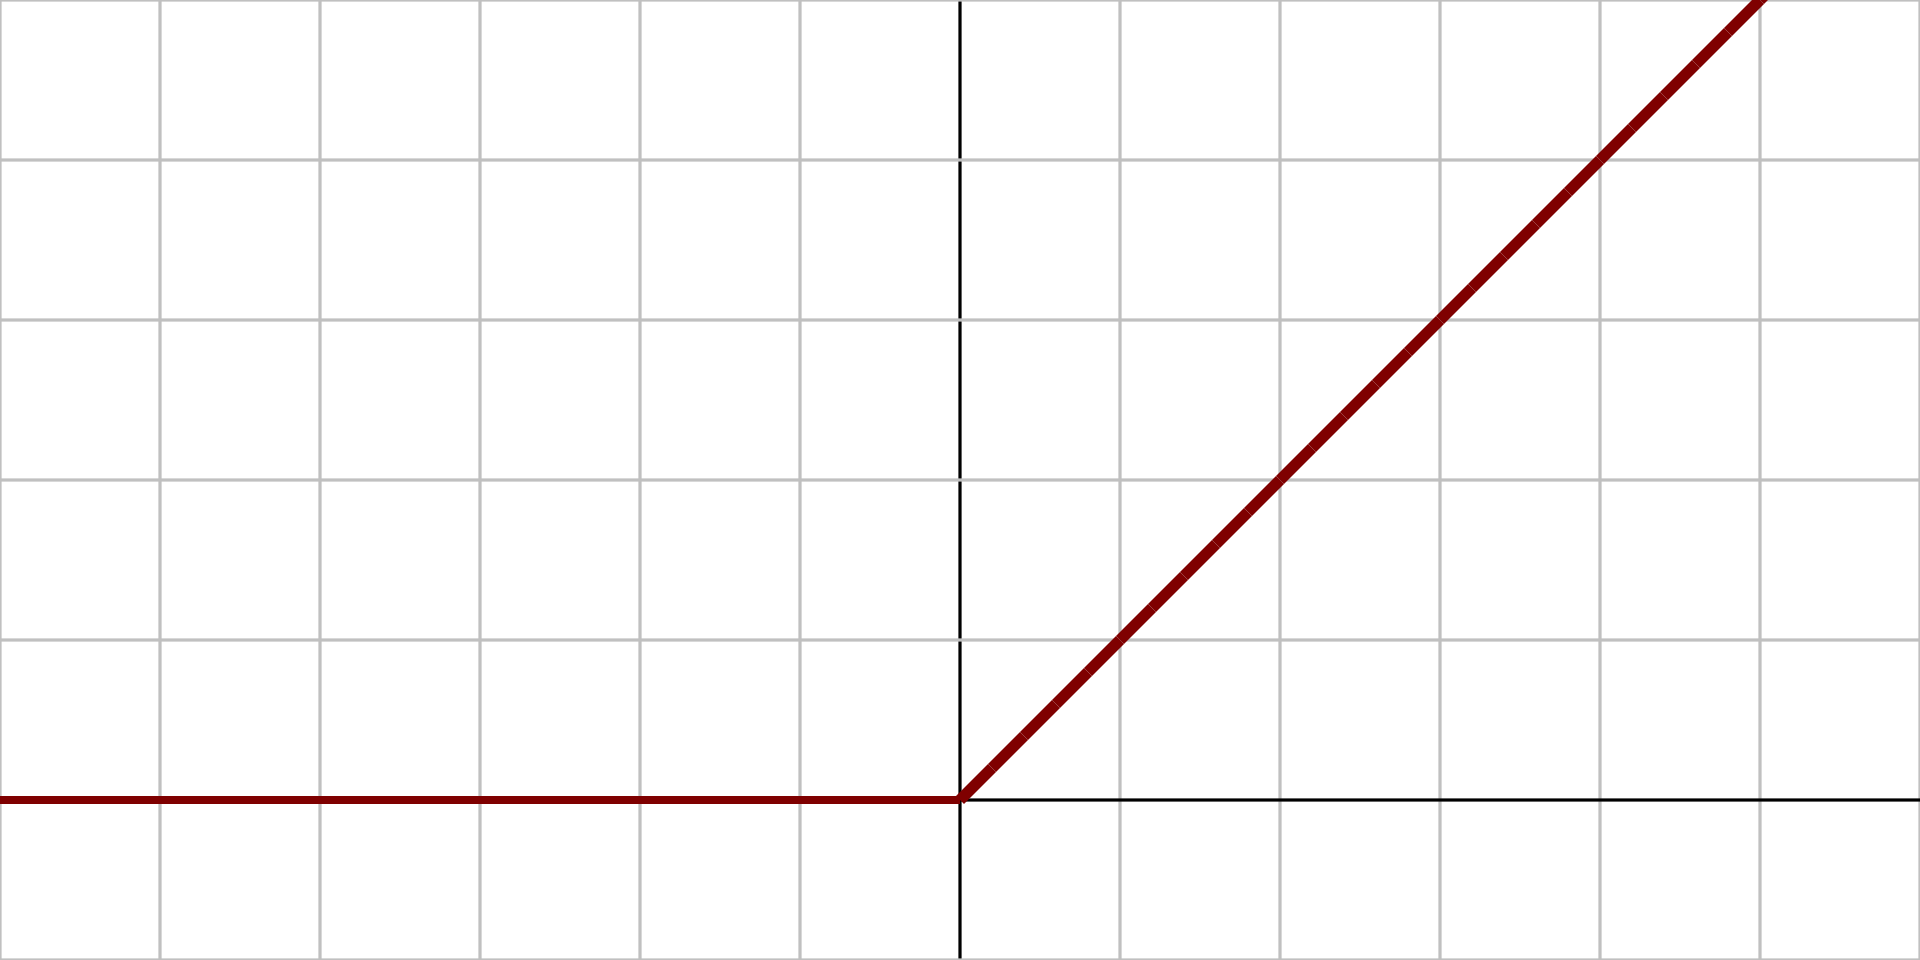
\includegraphics[width=0.5\linewidth]{relu}
	\caption[Rectified Linear Unit (ReLU)]{Rectified Linear Unit (ReLU). Source : tiré de \textit{Wikipedia}, ref. URL03}
	\label{fig:relu}
\end{figure}

\section{Perceptron Multicouche (PMC)}
\label{sec:3.3}

Un \gls{pmc} est une agrégation de couches cachées (couches entre les entrées et la sortie). Une couche est composée de perceptrons, ses entrées sont constituées de la sortie de la couche précédente (sauf pour la couche d'entrée) et sa sortie sera donc les entrées de la couche suivante.

\begin{figure}[H]
	\centering
	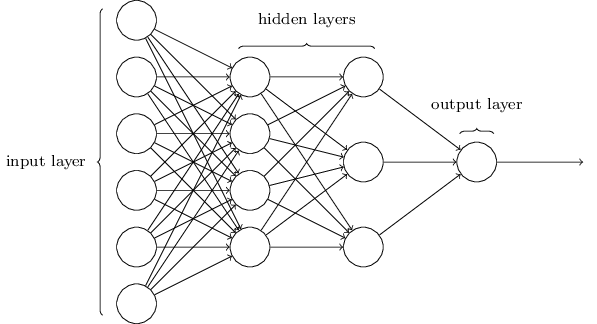
\includegraphics[width=0.7\linewidth]{pmc}
	\caption[Perceptron Multicouche (PMC)]{Perceptron Multicouche (PMC). Source : tiré de \textit{medium.com}, ref. URL04}
	\label{fig:pmc}
\end{figure}

Pour pouvoir corriger l’erreur sur les couches cachées, on utilise la technique de la rétropropagation du gradient. Le principe est d’effectuer la descente de gradient sur tous les vecteurs de poids du réseau et de propager l’erreur aux couches précédentes. Dans le cas où la fonction de coût est l’erreur quadratique et la fonction d’activation sigmoïde, la rétropropagation peut être décrite comme :

\begin{figure}[H]
	\centering
	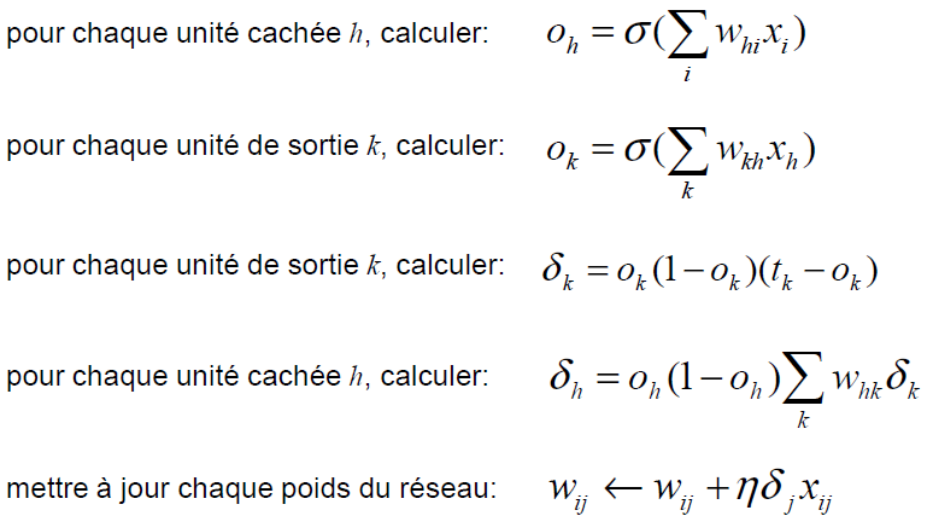
\includegraphics[width=0.7\linewidth]{backpropagation}
	\caption[Rétropropagation du gradient]{Rétropropagation du gradient. Source : tiré de \textit{l'Apprentissage Supervisé : Perceptrons Multicouche}, p. 18 / réalisé par \textsc{Bologna} Guido}
	\label{fig:retropropagation}
\end{figure}

\section{Couche de convolution}
\label{sec:3.4}

Dans le cas d'une couche de convolution, les entrées sont représentées différemment que pour le \gls{pmc}. Pour le \gls{pmc} nous avions un vecteur de valeurs réelles, la couche de convolution quant à elle prend un tenseur, c’est-à-dire un objet mathématique défini dans un espace vectoriel, et comme son nom l'indique, elle va appliquer un filtre dessus (convolution). Une couche convolutive est définie par plusieurs paramètres; il y a les canaux (filtres) qui représentent la dimension de l’espace d'entrée et de sortie de la couche, le noyau convolutif défini par sa largeur et sa hauteur (généralement symétriques) et le stride qui représente le pas de la convolution sur les dimensions.

\begin{figure}[H]
	\centering
	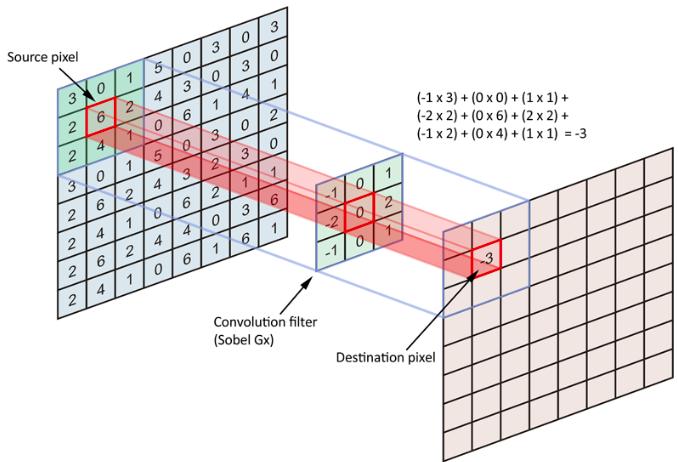
\includegraphics[width=0.7\linewidth]{convolutional_layer}
	\caption[Couche convolutive]{Couche convolutive. Source : tiré de \textit{medium.com}, ref. URL05 / réalisé par \textsc{Bui} Huy}
	\label{fig:conv_layer}
\end{figure}

\section{Couche d'agrégation}
\label{sec:3.5}

Une couche d’agrégation vient généralement après la couche de convolution et une couche de rectification (ReLU). Elle sert à résumer l’information et à diminuer le nombre de dimensions. Elle permet notamment d’éviter le surentrainement, de réduire le nombre de paramètres et de réduire la quantité de calculs nécessaires au réseau, mais surtout, elle rend le réseau invariant aux légères distorsions des données (par exemple pour la \gls{roc}, si le chiffre n’est pas situé au centre de l’image). Elle est définie par un noyau et un stride (comme pour la couche convolutive) puis par une fonction non linéaire qui va appliquer la transformation, la plus connue étant Max Pooling.

\begin{figure}[H]
	\centering
	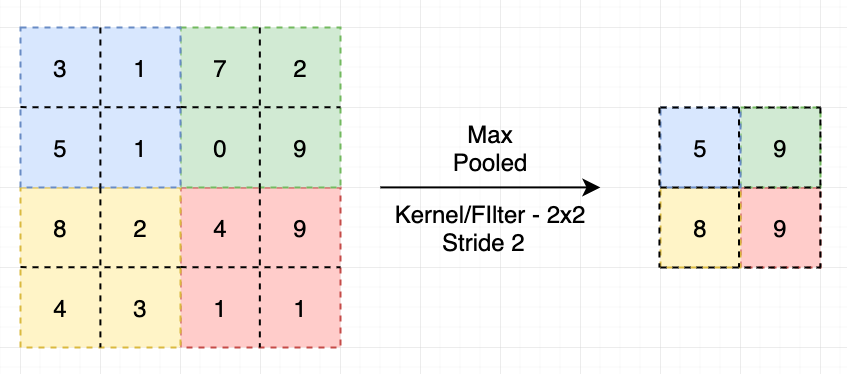
\includegraphics[width=0.7\linewidth]{pooling}
	\caption[Couche d'agrégation]{Couche d'agrégation. Source : tiré de \textit{ai.plainenglish.io}, ref. URL06 / réalisé par \textsc{Rana} Kartikeya}
	\label{fig:pooling}
\end{figure}

\section{Réseau Neuronal Convolutif (RNC)}
\label{sec:3.6}

Un \gls{rnc} est généralement utilisé dans les tâches avec des entrées fortement corrélées (la reconnaissance d'images, \gls{roc}, etc.). Dans notre cas, la détection de notes et accords de musique (séries chronologiques) présente des similarités suffisamment fortes pour qu'un \gls{rnc} semble être un choix approprié. Un \gls{rnc} possède une ou plusieurs couches convolutives entre les entrées et les couches inférieures du réseau.

\begin{figure}[H]
	\centering
	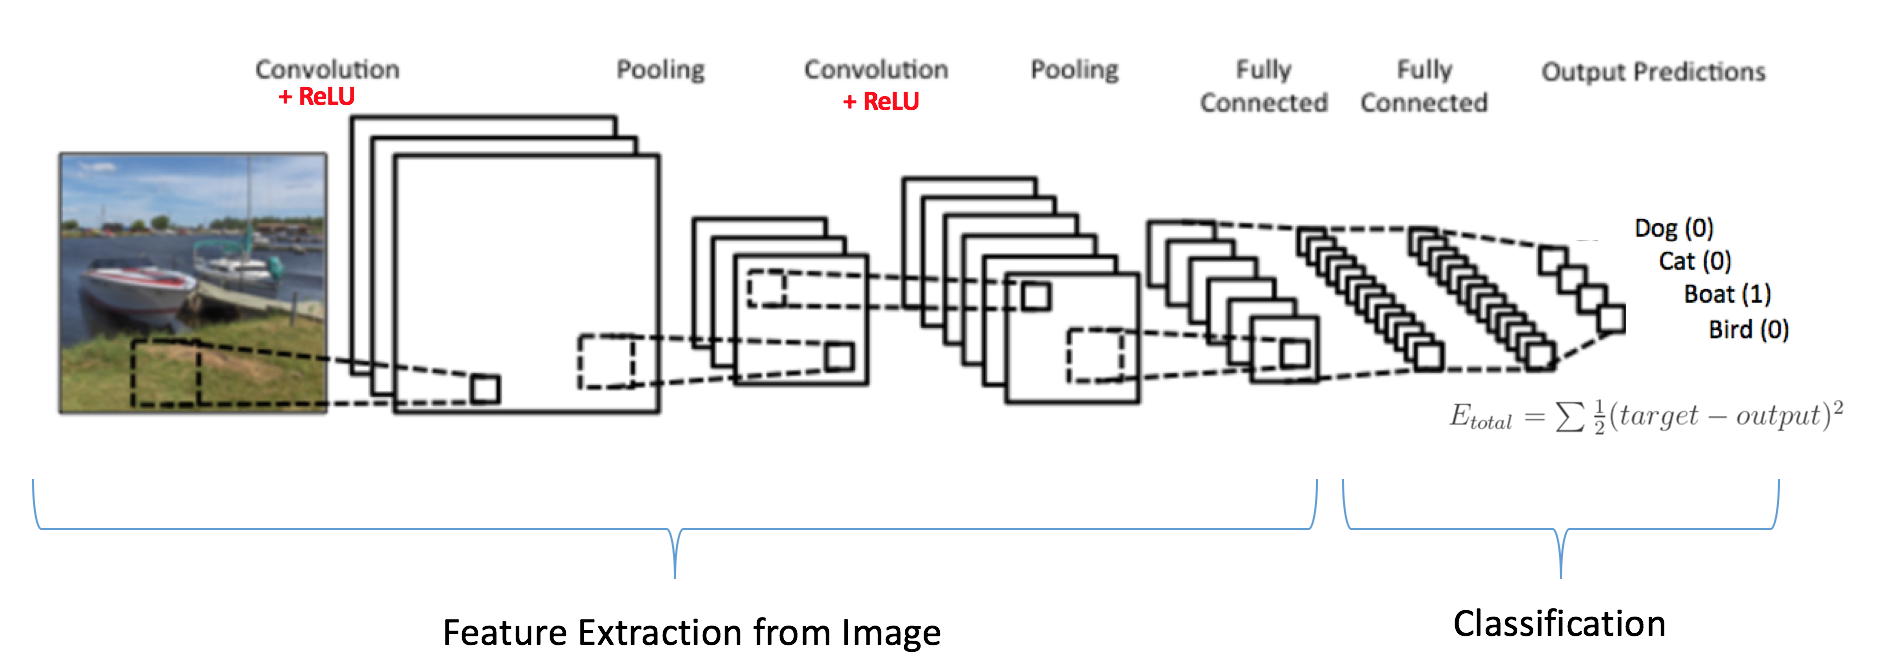
\includegraphics[width=1\linewidth]{rnc}
	\caption[Réseau Neuronal Convolutif (RNC)]{Réseau Neuronal Convolutif (RNC). Source : tiré de \textit{kdnuggets.com}, ref. URL07 / réalisé par \textsc{Ujiwal} Karn}
	\label{fig:rnc}
\end{figure}

Un \gls{rnc} peut avoir plusieurs classes en sortie (classement non-binaire); il faut donc un moyen de connaitre l’erreur pour chaque exemple. Pour cela, une fonction est appliquée à la couche de sortie, par exemple Softmax qui est une généralisation de la Sigmoïde et renvoie à un vecteur de probabilités sommant à un.

\begin{figure}[H]
	\centering
	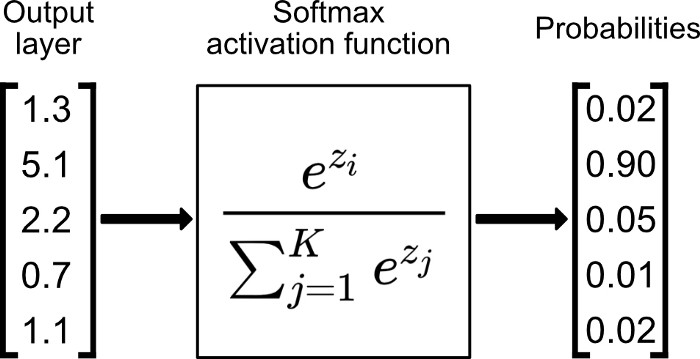
\includegraphics[width=0.5\linewidth]{softmax}
	\caption[Softmax]{Softmax. Source : tiré de \textit{towardsdatascience.com}, ref. URL08 / réalisé par \textsc{Radecic} Dario}
	\label{fig:softmax}
\end{figure}

Dans ce cas, la fonction de coût devient l’entropie croisée (somme des log-vraisemblances pour chaque classe) et elle peut se décrire comme :

\begin{figure}[H]
	\centering
	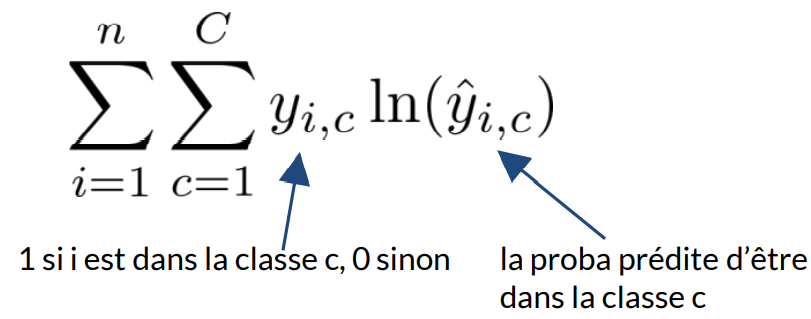
\includegraphics[width=0.5\linewidth]{cross_entropy}
	\caption[Entropie croisée]{Entropie croisée. Source : tiré de \textit{Les Réseaux Convolutifs}, p. 49 / réalisé par \textsc{Bologna} Guido}
	\label{fig:cross_entropy}
\end{figure}

\section{Long Short-Term Memory (LSTM)}
\label{sec:3.7}

Un \gls{lstm} est un type de \gls{rnr}. Une unité \gls{lstm} est généralement composée d’une cellule mémoire, d'une porte d’entrée, d'une porte de sortie et d'une porte d’oubli. Les réseaux \gls{lstm} sont de très bons réseaux lorsque l’on a des données chronologiques à traiter. Ils ont la possibilité d’oublier et de sauvegarder les données qui leur semblent utiles (extraction de caractéristiques ou \textit{features extraction} en anglais). Ils proposent aussi une solution au problème de la disparition du gradient qui est bien connu dans le domaine de l’apprentissage profond.

\begin{figure}[H]
	\centering
	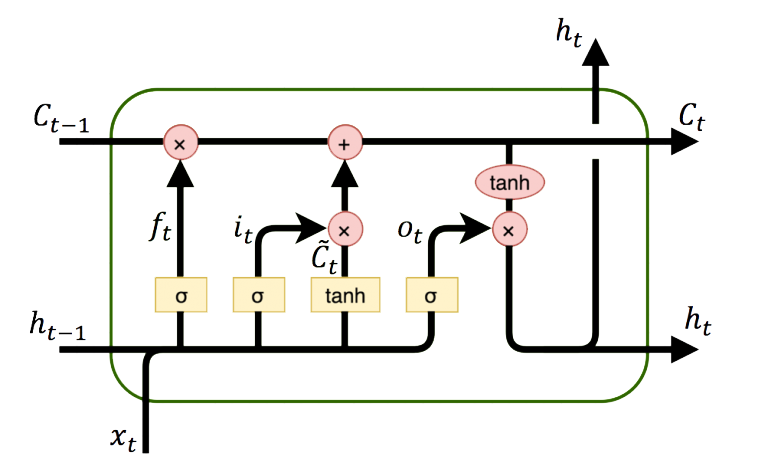
\includegraphics[width=0.7\linewidth]{lstm_cell}
	\caption[Long Short-Term Memory (LSTM)]{Long Short-Term Memory (LSTM). Source : tiré de \textit{apmonitor.com}, ref. URL09}
	\label{fig:lstm_cell}
\end{figure}

Dans les calculs suivants, nous ne tiendrons pas compte du biais. Le biais est tout simplement un neurone fictif (souvent égal à un). Il sert à décaler la fonction d’activation en y ajoutant une constante, cela aide à contrôler la valeur à laquelle la fonction d'activation s'activera.

\subsection{Porte d'oubli}

Lorsque l’on observe l’illustration \ref{fig:lstm_cell}, on remarque que la première opération effectuée est celle de la porte d’oubli. Avec $h_{t-1}$ étant l’état de la sortie à l’instant $t-1$, $X_{t}$ les entrées à l’instant $t$ et $W_{f}$ la matrice de poids, la porte d’oubli peut être décrite comme :

{\Large
	\setlength{\abovedisplayskip}{-0.5cm}
	\begin{gather*}
		f_{t} = \sigma(W_{f}[\overrightarrow{h}_{t-1}, \overrightarrow{x}_{t}])
	\end{gather*}
}

$f_{t}$ représente le vecteur d’oubli, c’est donc un vecteur de valeurs réelles entre zéro et un que l’on va multiplier avec le vecteur $C_{t-1}$, qui lui représente le vecteur de mémoire à l’instant $t-1$.

\subsection{Porte d'entrée}

La porte d’entrée quant à elle se décompose en deux parties, une première appliquant la Sigmoïde sur notre vecteur de valeurs et la deuxième qui applique Tanh.

La sortie $i_{t}$ de la sigmoïde représente un vecteur de valeurs réelles entre zéro et un. Il représente la quantité (l’importance) d’informations que l’on va garder. Avec $W_{i}$ une matrice de poids, cette partie peut être définie comme :

{\Large
	\setlength{\abovedisplayskip}{-0.5cm}
	\begin{gather*}
		i_{t} = \sigma(W_{i}[\overrightarrow{h}_{t-1}, \overrightarrow{x}_{t}])
	\end{gather*}
}

La sortie de Tanh va être un vecteur de valeurs réelles entre moins un et un. Cela correspond en quelque sorte à un vecteur de proposition, il représente les données que l’on va garder lors de la multiplication avec le vecteur $i_{t}$. Avec $W_{c}$ une matrice de poids, cette partie peut être définie comme :

{\Large
	\setlength{\abovedisplayskip}{-0.5cm}
	\begin{gather*}
		\tilde{C}_{t} = \text{Tanh}(W_{c}[\overrightarrow{h}_{t-1}, \overrightarrow{x}_{t}])
	\end{gather*}
}

\subsection{Cellule mémoire}

La cellule mémoire est toute simple, il s’agit uniquement d’un calcul où l’on multiplie le vecteur mémoire de l’état précédent ($C_{t-1}$) au vecteur d’oubli ($f_{t}$) puis on lui ajoute les nouvelles données.

{\Large
	\setlength{\abovedisplayskip}{-0.5cm}
	\begin{gather*}
		C_{t} = (C_{t-1}\times f_{t}) + (i_{t}\times\tilde{C}_{t})
	\end{gather*}
}

\subsection{Porte de sortie}

La porte de sortie se décompose également en deux étapes, une première où l’on applique la Sigmoïde sur notre vecteur de valeurs réelles, puis une deuxième où l'on multiplie la sortie de la Sigmoïde par le Tanh de notre mémoire à l’instant $t$.

Lors de la première partie, exactement comme pour la porte d’entrée, on va définir la quantité (l’importance) d’informations que l’on va garder pour notre sortie. Avec une matrice $W_{o}$, cette partie peut être décrite comme :

{\Large%
	\setlength{\abovedisplayskip}{-0.5cm}
	\begin{gather*}
		o_{t} = \sigma(W_{o}[\overrightarrow{h}_{t-1}, \overrightarrow{x}_{t}])
	\end{gather*}
}%

Pour finir, la sortie de notre unité à l’instant $t$ ($h_{t}$) est tout simplement définie comme :

{\Large%
	\setlength{\abovedisplayskip}{-0.5cm}
	\begin{gather*}
		h_{t} = o_{t}\times\text{Tanh}(C_{t})
	\end{gather*}
}%
